\section{Experiments}
In this section, we report our reproduction effort and verification of the experimental results in the paper.

\subsection{Toy Example}

We first reproduced the toy example about 1D Gaussian mixture mentioned in the paper. 

\begin{figure}[h]
    \centering
    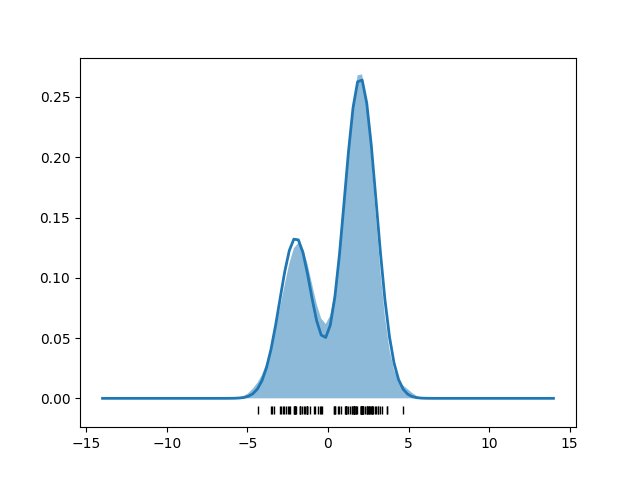
\includegraphics[width=\textwidth]{original-code/Toy-Examples/mixture1d_iter_500.png}
    \caption{Toy example with 1D Gaussian mixture}
    \label{fig:my_label}
\end{figure}

\begin{figure}[h]
    \centering
    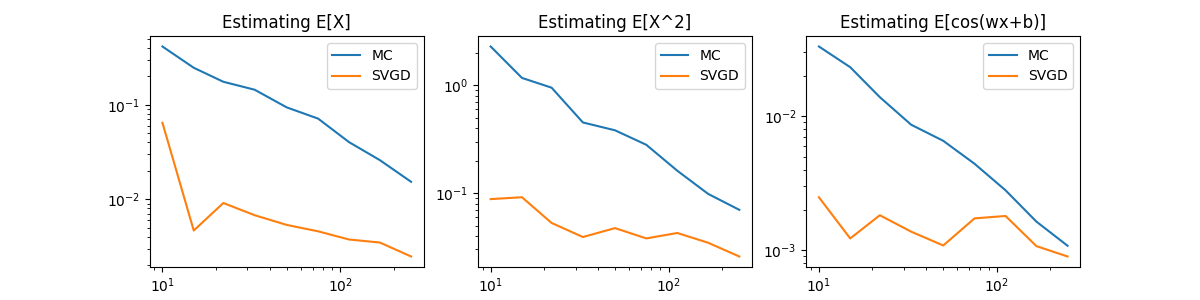
\includegraphics[width=\textwidth]{figs/toy-figure2.png}
    \caption{Comparison between MC and SVGD on simple mean estimation tasks}
    \label{fig:my_label}
\end{figure}

\subsection{Bayesian Logistic Regression}

\begin{figure}[h]
    \centering
    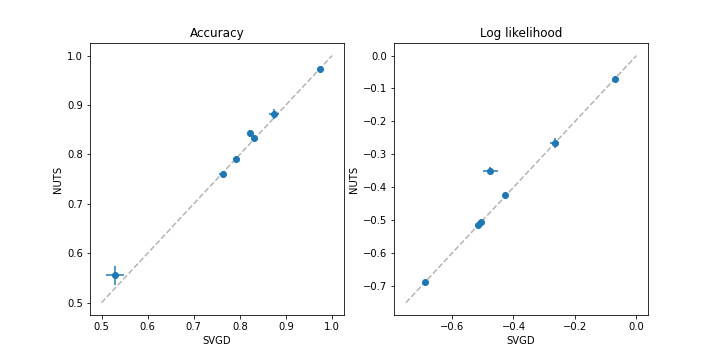
\includegraphics[width=\textwidth]{figs/logistic_svgd_nuts.png}
    \caption{Caption}
    \label{fig:my_label}
\end{figure}

\subsection{Bayesian Neural Network}

A Bayesian Neural Network (BNN) is a neural network where 

For the experiments, we train a small BNN on a set of regression tasks. We follow the setup from the paper and use the UCI dataset. We run tests on the SVGD algorithm as implemented by the authors of the original paper and also the implementation on NumPyro, and also on the probabilistic back-propagation (PBP) algorithm. A change that we made was to run each algorithms using the same batch size and the same number of epochs ran across all of the tests.

\begin{table}[]
    \centering
\begin{tabular}{|c|ccc|}
\hline
 Dataset & PBP & SVGD (NumPyro) & SVGD (original)  \\
 \hline
boston & $3.039 \pm 0.303$ & $3.430 \pm 0.449$ & $2.999 \pm 0.343$ \\
concrete & $5.699 \pm 0.075$ & $5.661 \pm 0.145$ & $5.763 \pm 0.090$ \\
energy & $1.676 \pm 0.050$ & $1.143 \pm 0.064$ & $1.421 \pm 0.049$ \\
kin8nm & $0.099 \pm 0.001$ & $0.077 \pm 0.001$ & $0.121 \pm 0.001$ \\
naval & $0.006 \pm 0.000$ & $0.001 \pm 0.000$ & $0.008 \pm 0.000$ \\
power & $4.143 \pm 0.050$ & $4.156 \pm 0.051$ & $4.206 \pm 0.049$ \\
protein & $4.680 \pm 0.009$ & $4.518 \pm 0.009$ & $4.859 \pm 0.013$ \\
wine & $0.640 \pm 0.015$ & $0.666 \pm 0.013$ & $0.634 \pm 0.014$ \\
yacht & $0.948 \pm 0.087$ & $1.719 \pm 0.101$ & $1.017 \pm 0.141$ \\
\hline
\end{tabular}
    \caption{Caption}
    \label{tab:my_label}
\end{table}

In our results, we found that the SVGD algorithm was not able to exactly matc

\begin{figure}[h]
    \centering
    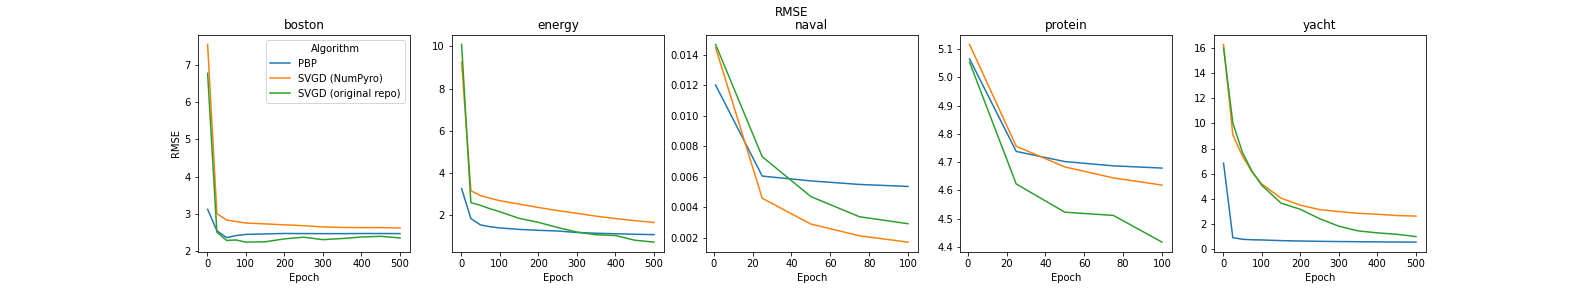
\includegraphics[width=\textwidth]{figs/bayesian_epoch_RMSE.png}
    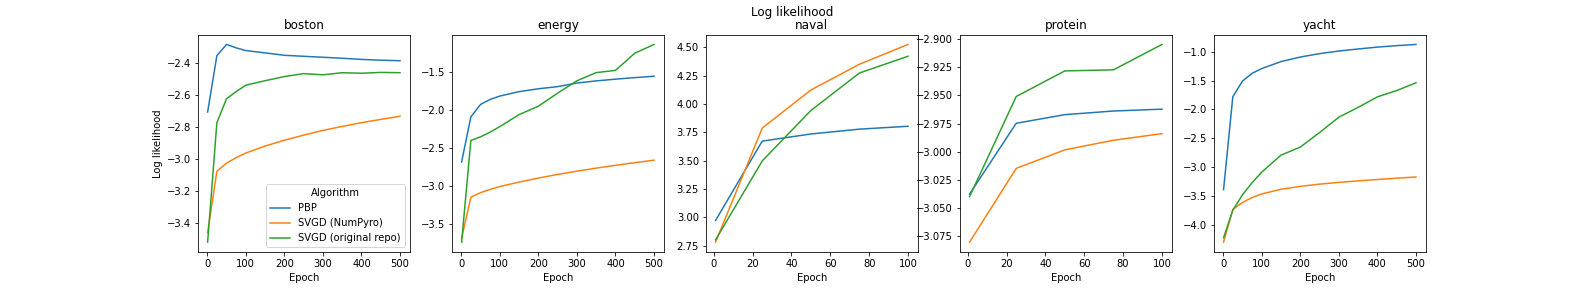
\includegraphics[width=\textwidth]{figs/bayesian_epoch_Loglikelihood.png}
    \caption{Caption}
    \label{fig:my_label}
\end{figure}